%%%%%%%%%%%%%%%%%%%%%%%%%%%%%%%%%%%%%%%%%%%%%%%%%%%%%%%%%%%%%%%%%%%%%%
% How to use writeLaTeX: 
%
% You edit the source code here on the left, and the preview on the
% right shows you the result within a few seconds.
%
% Bookmark this page and share the URL with your co-authors. They can
% edit at the same time!
%
% You can upload figures, bibliographies, custom classes and
% styles using the files menu.
%
% If you're new to LaTeX, the wikibook is a great place to start:
% http://en.wikibooks.org/wiki/LaTeX
%
%%%%%%%%%%%%%%%%%%%%%%%%%%%%%%%%%%%%%%%%%%%%%%%%%%%%%%%%%%%%%%%%%%%%%%
\documentclass{tufte-handout}

%\geometry{showframe}% for debugging purposes -- displays the margins

\usepackage{amsmath}

% Set up the images/graphics package
\usepackage{graphicx}
\setkeys{Gin}{width=\linewidth,totalheight=\textheight,keepaspectratio}
\graphicspath{{graphics/}}

\title{Formula Evaluation}
\author{Abraham Hinteregger}
%\date{24 January 2009}  % if the \date{} command is left out, the current date will be used

% The following package makes prettier tables.  We're all about the bling!
\usepackage{booktabs}

% The units package provides nice, non-stacked fractions and better spacing
% for units.
\usepackage{units}

% The fancyvrb package lets us customize the formatting of verbatim
% environments.  We use a slightly smaller font.
\usepackage{fancyvrb}
\fvset{fontsize=\normalsize}

% Small sections of multiple columns
\usepackage{multicol}

% Provides paragraphs of dummy text
\usepackage{lipsum}


\usepackage{amssymb}
\usepackage{wrapfig}
\usepackage{amsmath}
\usepackage[english]{babel}
\usepackage[utf8]{inputenc}
\usepackage{float}
\usepackage{graphicx}
%\usepackage{wrapfig}
\usepackage{textcomp}
\usepackage{braket}
\usepackage{bbm}
\usepackage{framed}
\usepackage{ifthen}
\usepackage{bbold}
\usepackage{colortbl}
\usepackage{xifthen}
\usepackage{color}
\usepackage{ifthen}
\usepackage[T1]{fontenc}
\usepackage{amsthm}
\usepackage{bm}
\usepackage{amsbsy}
\usepackage{tikz}
\usepackage{xspace}
\usepackage{fancyref}

\usepackage{xcolor}
\usepackage{scalefnt}
\usepackage{caption}
\newcommand{\V}{\ensuremath{\mathbf{V}}\xspace}
\newcommand{\F}{\ensuremath{\mathbf{F}}\xspace}

% These commands are used to pretty-print LaTeX commands
\newcommand{\doccmd}[1]{\texttt{\textbackslash#1}}% command name -- adds backslash automatically
\newcommand{\docopt}[1]{\ensuremath{\langle}\textrm{\textit{#1}}\ensuremath{\rangle}}% optional command argument
\newcommand{\docarg}[1]{\textrm{\textit{#1}}}% (required) command argument
\newenvironment{docspec}{\begin{quote}\noindent}{\end{quote}}% command specification environment
\newcommand{\docenv}[1]{\textsf{#1}}% environment name
\newcommand{\docpkg}[1]{\texttt{#1}}% package name
\newcommand{\doccls}[1]{\texttt{#1}}% document class name
\newcommand{\docclsopt}[1]{\texttt{#1}}% document class option name

\usetikzlibrary{trees}
\usetikzlibrary{positioning}
\tikzset{main node/.style={circle,fill=black,draw,minimum size=3pt,inner sep=0pt},}

\begin{document}

\maketitle% this prints the handout title, author, and date

\begin{abstract}
\noindent Game semantics can be used as didactic approach to logics that is more accessible than the usual model theoretic semantics. Furthermore it allows extending logics with ideas inherent to games that don't have a direct correspondence in logics -- taking logics from propositional statements to dynamic activities.
\end{abstract}

%\printclassoptions

\section{The game ``$game(M,s,\varphi)$''}
The game can be visualized as a tree where at every node one of the two players is active and chooses the branch where the game continues. A node consists of the state of the game at the current point, depending on the logics used this consists of the model $M$, a variable setting $s$, the current formula $\varphi$ and (in case in case of modal logics) the current world $w$.
The outermost operator of the formula defines which player is active and which moves are available.
\\
\textcolor{white}{x}\\

\marginnote[0.4cm]{$w$ only for modal logics} 
\marginnote[0.1cm]{The logical constants $\top,\bot$ are atoms} 
\marginnote[1.0cm]{Switching of strategies follows from this} 
\begin{tabular}{cl}
$\varphi$ & Interpretation of $game(M,s,[w,]\varphi)$\\\hline
atomic &  \V wins if $M,s\models \text{[atom]}$, else \F wins\\
$\varphi_1 \lor \varphi_2$ & \V chooses which disjunct to play. $\rightarrow game(M,s,\varphi_i)$\\
   $\varphi_1 \land \varphi_2$ & \F chooses which conjunct to play. $\rightarrow game(M,s,\varphi_i)$\\
  $ \lnot \varphi$ & reverse win markings $\rightarrow game(M,s,\varphi)$\\\\
  $\exists x ; \varphi$ & \V  assigns object to $x$: $\rightarrow game(M,s[x:=d],\varphi)$\\
  $\forall x ; \varphi$& \F assigns object to $x$:  $\rightarrow game(M,s[x:=d],\varphi)$\\\\
 $\Box \varphi$ & \F chooses a successor $v$ of $w$: $\rightarrow game(M,s,v,\varphi)$\\
 $\Diamond \varphi$ & \V chooses a successor $v$ of $w$: $\rightarrow game(M,s,v,\varphi)$\\\\
\end{tabular}

If either player can't move (i.e.: no possible successor for the current world) he loses.
\subsection{Success Lemma}
\V has a winning strategy for $game(M,s\varphi)$ if and only if $M,s\models\varphi$\marginnote{The same holds for \F}

\subsection{Example of modal game}
In \fref{fig:fig1} is an example for a modal logic game. It contains most of the elements outlined above. \V has a winning strategy but could also lose if he wants to.

\tikzstyle{level 1}=[level distance=2.5cm, sibling distance=6cm]
\tikzstyle{level 2}=[level distance=2.5cm, sibling distance=3cm]

% Define styles for bags and leafs
\tikzstyle{bag} = [text width=4em, text centered]
\tikzstyle{end} = [circle, minimum width=3pt,fill, inner sep=0pt]

\begin{figure*}
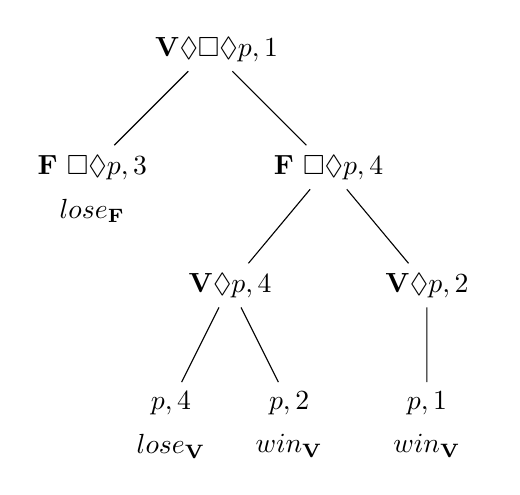
\begin{tikzpicture}[grow=down, sloped]
% Set the overall layout of the tree
\tikzstyle{level 1}=[level distance=1.5cm, sibling distance=3cm]
\tikzstyle{level 2}=[level distance=1.5cm, sibling distance=2.5cm]
\tikzstyle{level 3}=[level distance=1.5cm, sibling distance=1.5cm]
% Define styles for bags and leafs
\tikzstyle{bag} = [text width=4em, text centered]
\tikzstyle{end} = [circle, minimum width=3pt,fill, inner sep=0pt]



\node[bag] { ${\V\Diamond\Box\Diamond p,1}\quad $}
    child {node[bag,label=below:{$lose_\F$}] {\F $\Box\Diamond p, 3$}}
    child {node[bag] { ${\F\ \Box\Diamond p, 4}$}        
	child {node[bag] {{$\V \Diamond p, 4$}}
		child {node[bag, label=below:{$lose_\V$}] {$p, 4$}}
		child {node[bag, label=below:{$win_\V$}] {$p, 2$}}
	}
	child {node[bag] {$\V \Diamond p, 2$}
		child {node[bag, label=below:{$win_\V$}] {$p, 1 $}}
          }
   };

\end{tikzpicture}
\begin{tikzpicture}[grow=down, sloped]

 \node[main node,label=left:{1 $p$}] (1) {};
    \node[main node,label=left:{3}] (3) [below of = 1]  {};
    \node[main node,label=right:{2 $p$}] (2) [right = 1.5cm of 1] {};
    \node[main node,label=right:{4}] (4) [below of = 2] {};
     \path[-latex,draw,thick]    (2) edge node {} (1);
     \path[-latex,draw,thick]    (1) edge node {} (3);
     \path[-latex,draw,thick]    (4) edge node {} (2);
     \path[-latex,draw,thick]    (1) edge node {} (4);
     \path[-latex,draw,thick]    (4) edge [out=300,in=240,looseness=30] node {}(4);
  
  
  %ugly hacks follow
\node[opacity=0](y) [below = 3 cm of 1]{}; % some spacing above 
\node[opacity=0](x) [left = 2.5cm of 1]{}; % for centering
\end{tikzpicture}
\caption{Game tree for $game(M,s,1,\Diamond\Box\Diamond p)$ on the left, accessibility relations and Kripke interpretation on the right.}\label{fig:fig1}

\end{figure*}



\section{Modal $\mu$-calculus}
Extends modal logic with least ($\mu p : \varphi(p)$) and greatest ($\nu p : \varphi(p)$) fixpoint operator. $p$ must occur positively\footnote{even mount of $\lnot$ in front of $p$} in $\varphi(p)$. A world $w$ is within the set defined by $\mu p : \varphi(p)$ iff $M,w\models \varphi(p)$ or there's a finite expansion of $\varphi(p)$ s.t. $M,w\models\varphi(\ldots(\varphi(p)))$.

$\nu$ also allows infinite expansions.
\subsection{Evaluation game for $\mu$-calculus}
\begin{tabular}{cl}
$\varphi$ & Interpretation of $game(M,s,w,\varphi)$\\\hline
$\nu p: \varphi(p)$ &  game proceeds with $game(M,s,w,\varphi(p))$\\
$p$ & formula to which $p$ is bound is substituted back in for p\\
& game proceeds with $game(M,s,w,\varphi(p))$\\\\
\end{tabular}
If the game has infinite loops \V wins if the highest ranked fixed point formula is a $\nu$ formula and \F wins if it's a $\mu$ formula.\marginnote{The rank of a formula is higher than the rank of its subformulas}
\nocite{*}
\bibliographystyle{plainnat}
\bibliography{loghandout}



\end{document}